%%%%%%%%%%%%%%%%%%%%%%%%%%%%%%%%%%%%%%%%%%%%%%%%%%%%%%%%%%%
% | - Active Learning Machine Learning Results
% %%%%%%%%%%%%%%%%%%%%%%%%%%%%%%%%%%%%%%%%%%%%%%%%%%%%%%%%%
%
% __|
%%%%%%%%%%%%%%%%%%%%%%%%%%%%%%%%%%%%%%%%%%%%%%%%%%%%%%%%%%%



% %%%%%%%%%%%%%%%%%%%%%%%%%%%%%%%%%%%%%%%%%%%%%%%%%%%%%%%%%
% | - Intro To Section
% Intro/transition paragraph
% __|
% %%%%%%%%%%%%%%%%%%%%%%%%%%%%%%%%%%%%%%%%%%%%%%%%%%%%%%%%%
% | - PARAGRAPH BODY
%
We next applied the AL algorithm to the discovery of stable and unique polymorphs of \IrOtwo and \IrOthree, individually.
%
Results for \IrOtwo are provided in the supporting information (Figure \ref{fig:iro2_al}), here we focus on \IrOthree,
since it is a comparatively unexplored oxide system.

%and here we will illustrate the results for \IrOthree only,
%since it is a comparatively unexplored oxide system.
%
% TODO I don't talk about IrO2 enough
%We will briefly touch on the results for \IrOtwo at the end and refer the reader to the Supporting Information for further details (Figure \ref{fig:iro2_al}).
% __|
%%%%%%%%%%%%%%%%%%%%%%%%%%%%%%%%%%%%%%%%%%%%%%%%%%%%%%%%%%%


% %%%%%%%%%%%%%%%%%%%%%%%%%%%%%%%%%%%%%%%%%%%%%%%%%%%%%%%%%
% | - AL Results for IrO3
% * Introduce the convergence plots
% * The GP becomes more accurate as more DFT is acquired
% * The GP can start to recognize the low energy systems after minimal DFT
%
% We need to call them something else than "convergence plots" (bad name)
% __|
% %%%%%%%%%%%%%%%%%%%%%%%%%%%%%%%%%%%%%%%%%%%%%%%%%%%%%%%%%
% | - PARAGRAPH BODY
%
Figure~\ref{fig:iro3_al}a, shows a sequence of snapshots of the AL algorithm applied to \IrOthree at different generations.
%
Each subplot reports the predicted (grey) and DFT-derived (filled red) formation enthalpies (\DHf) for each structure, sorted by stability such that structures more likely to be selected by the acquisition criteria are farther left.
%
As the algorithm acquires DFT data, the GP model's accuracy increases,
as evidenced by the decreasing uncertainties when comparing the initial and latter generations (\ref{fig:iro3_al}a.i-v).
%
At the top of each subplot of Figure~\ref{fig:iro3_al}a the x-axis positioning of the ten most stable polymorphs is tracked.
%
Initially, these ten structures are randomly distributed across the entire candidate space due to the lack of training data for the GP model.
%
However, after only three generations (Figure~\ref{fig:iro3_al}a.ii) the GP model is sufficiently accurate to predict the most stable polymorphs as low energy structures.
%
By the fifth generation (\num{30} DFT relaxations) \num{4/10} of the most stable polymorphs have been acquired,
including the globally stable phase of \IrOthree, which
was found on average in only 4 generations (averaged over 100 independent runs).
%
By the 14th generation of the AL,
\num{9/10} of the most stable structures were acquired.
% __|
%%%%%%%%%%%%%%%%%%%%%%%%%%%%%%%%%%%%%%%%%%%%%%%%%%%%%%%%%%%


% %%%%%%%%%%%%%%%%%%%%%%%%%%%%%%%%%%%%%%%%%%%%%%%%%%%%%%%%%
% | - Paragraph About Structures Found
% How to balance this with the next section that has more details on structural stuff?
% __|
% %%%%%%%%%%%%%%%%%%%%%%%%%%%%%%%%%%%%%%%%%%%%%%%%%%%%%%%%%
% | - PARAGRAPH BODY
%
Seven of the most stable \IrOthree polymorphs discovered are shown in Figure~\ref{fig:iro3_al}b.
%
All of the low energy \IrOthree structures are constructed from octahedrally coordinated units, with a variety of symmetries and packing modes.
%
The globally stable crystal structure consists of a six-atom primitive cell with a space group number of \num{167} (R$\overline{3}$c) in the rhombohedral crystal system, has exclusively corner-sharing octahedra, and is isomorphic to \ce{FeF_{3}}~\cite{Hepworth1957}.
%
Herein, this structure will be referred to as \aIrOthree.
%
The second most stable polymorph (Figure~\ref{fig:iro3_al}b.ii) is similar to \aIrOthree,
only differing by the stacking of the alternating layers orthogonal to the \textbf{c} lattice vector.
%
We label this structure $\alpha_{2}$-\ce{IrO_3} in Figure~\ref{fig:iro3_al}b and it is only 2 meV/atom less stable than \aIrOthree, well within the margin of error for DFT.
%
The fourth most stable structure (\rIrOthree) is notable for being the first in the series to have mixed edge- and corner-sharing octahedra and is structurally similar to rutile (\rIrOtwo).
% __|
%%%%%%%%%%%%%%%%%%%%%%%%%%%%%%%%%%%%%%%%%%%%%%%%%%%%%%%%%%%


% %%%%%%%%%%%%%%%%%%%%%%%%%%%%%%%%%%%%%%%%%%%%%%%%%%%%%%%%%
% | - Performance of AL Model
%
% __|
% %%%%%%%%%%%%%%%%%%%%%%%%%%%%%%%%%%%%%%%%%%%%%%%%%%%%%%%%%
% | - PARAGRAPH BODY
%
Figure~\ref{fig:iro3_al}c reports the discovery rate of the AL algorithm by plotting
the number of the ten most stable systems acquired against the number of DFT calculations with the GP-LCB acquisition and a random acquisition scheme to serve as a baseline.
%
The results of Figure~\ref{fig:iro3_al}c are averaged over \num{100} independent runs of the AL algorithms with the standard deviation shown.
%
Overall, the GP-LCB runs outperform the random acquisition runs, with on average only \num{100} DFT calculations needed to discover the ten most stable structures.
%
This demonstrates over a factor of two improvement in performance compared to random acquisition, which does not acquire the most stable structures until all candidates are computed.
%
The results for \IrOtwo (Figure \ref{fig:iro2_al}) show a higher discovery rate for GP-LCB compared to the random acquisition method,
although the GP-LCB method ``saturated'' at \num{9/10} and was unable to acquire the last structure until the candidate space was exhausted.
%
The performance of GP-LCB relative to random is expected to increase with the size of the candidate space, since the probability of selecting stable structures is inversely proportional to the size of the candidate pool.
% __|
%%%%%%%%%%%%%%%%%%%%%%%%%%%%%%%%%%%%%%%%%%%%%%%%%%%%%%%%%%%


% =========================================================
% FIGURE ==================================================
% =========================================================
% | - Figure | IrO3 Convergence Plot
\begin{figure*}[!htb]
\centering
\makebox[\textwidth][c]{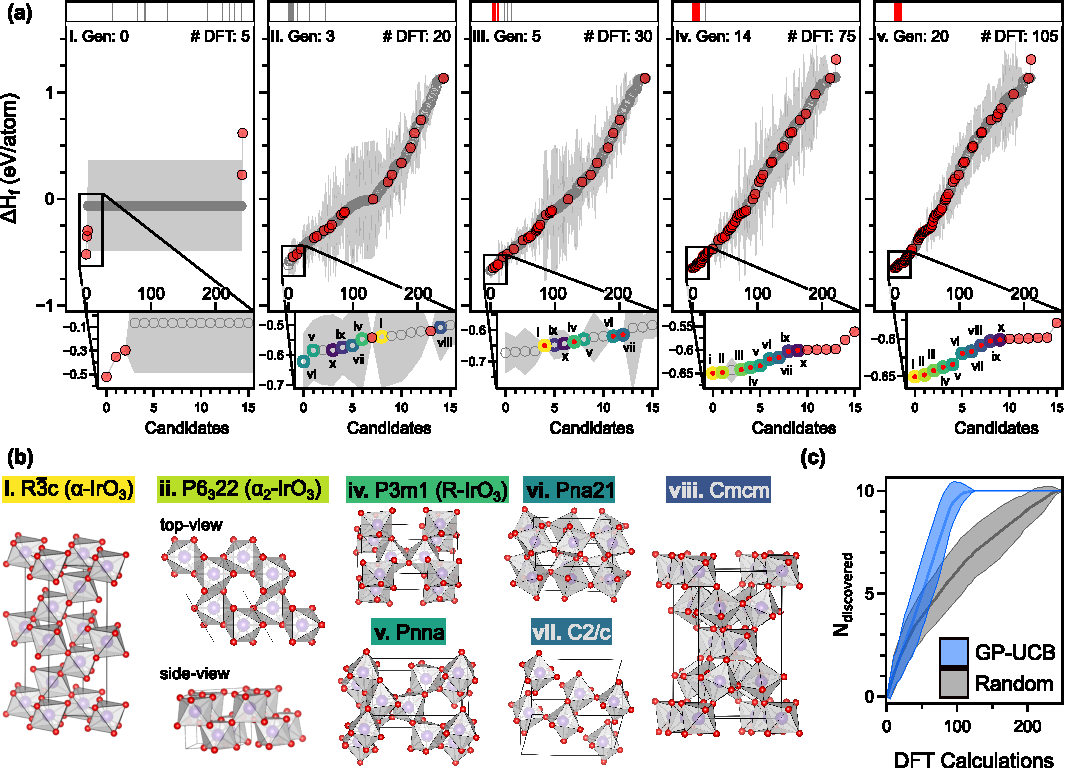
\includegraphics[width=\textwidth,height=\textheight,keepaspectratio]
{02_figures/ml_convergence_plots/00_ml_plot_iro3_al__v16__downsampled_0900x0900.pdf}}
\caption{\label{fig:iro3_al}
% (a) %%%%%%%%%%%%%%%%%%%%%%%%%%%%%%%%%%%%%%%%%%%%%%%%%%%%%
%
(a) The state of the AL algorithm at five generations.
%
The enthalpy of formation per atom (\DHf) is plotted, ordered by stability, against all \IrOthree candidates, with the 1 $\sigma$ uncertainty estimate shown for each prediction.
%
The number of DFT training points at each generation is displayed.
%
Hollow grey markers indicate a GP model predicted \DHf while red indicate a DFT-computed quantity.
%
At the top of subplots a.i - a.v, the x-axis positions of the ten most stable polymorphs are tracked at each generation by either red (acquired) or grey (not acquired) vertical lines.
%
Insets of the low energy region for each generation is displayed below each subplot.
%
The top ten most stable systems are colored and labeled (i-vii) to indicate their identity.
% (b) %%%%%%%%%%%%%%%%%%%%%%%%%%%%%%%%%%%%%%%%%%%%%%%%%%%%%
%
(b) Crystal structures of the \num{8} most stable \IrOthree polymorphs (structure iii. not shown).
%
% (c) %%%%%%%%%%%%%%%%%%%%%%%%%%%%%%%%%%%%%%%%%%%%%%%%%%%%%
%
(c) The number of most stable \num{10} polymorphs of \IrOthree discovered vs. the number of DFT calculations for the GP-LCB (blue) and random (grey) acquisition methods.
%
The results are averaged over \num{100} independent runs and the 1 $\sigma$ standard deviation between these runs are displayed.
}
\end{figure*}
% __| =====================================================
% =========================================================


% %%%%%%%%%%%%%%%%%%%%%%%%%%%%%%%%%%%%%%%%%%%%%%%%%%%%%%%%%
% | - Parity Plot Discussion
% Discussion on performance of the AL routine
% __|
% %%%%%%%%%%%%%%%%%%%%%%%%%%%%%%%%%%%%%%%%%%%%%%%%%%%%%%%%%
% | - PARAGRAPH BODY
We next evaluate the prediction accuracy of the \IrOtwo and \IrOthree GP regression models utilizing the full DFT optimized data set of 487 \IrOtwo and 249 \IrOthree structures.
%
This dataset corresponds to the final generation of the AL algorithm in which all structures have been acquired.
%
Figure~\ref{fig:parity} plots the GP model predicted \DHf against the DFT-computed values for two cases.
%
Case 1) shows the predictions on the structural fingerprints prior to DFT-optimization (grey), as is done in the regular operation of the algorithm.
%
Case 2) shows the prediction of the same GP model using the post-DFT optimized fingerprints (blue) with \num{10}-fold cross-validation.
%
It is evident that using the pre-optimization fingerprints results in the GP model being inaccurate in quantitatively predicting the post-relaxation DFT formation energy of the candidate space,
with a seemingly large MAE of \mytilde\num{1.5} eV/atom.
%
In contrast, the same GP model does comparatively much better at predicting the formation energies of post-DFT optimized structures with an MAE of \mytilde\num{0.2} eV/atom.
% __|
%%%%%%%%%%%%%%%%%%%%%%%%%%%%%%%%%%%%%%%%%%%%%%%%%%%%%%%%%%%


% %%%%%%%%%%%%%%%%%%%%%%%%%%%%%%%%%%%%%%%%%%%%%%%%%%%%%%%%%
% | - Detailed Analysis of Pre vs. Post DFT Predictions
%
% __|
% %%%%%%%%%%%%%%%%%%%%%%%%%%%%%%%%%%%%%%%%%%%%%%%%%%%%%%%%%
% | - PARAGRAPH BODY
%
%The apparent discrepancy between the predictive capability on structures fingerprinted before and after relaxation is intriguing in terms of the general utility of AL in DFT datasets,
%and has implications on the effectiveness of our approach.
%
%Additionally, 
The drastic decrease in prediction error is not surprising,
since the post-DFT fingerprints directly correspond to the target \DHf values,
and is primarily due to the large degree of structural drift that occurs during DFT relaxation,
the extent of which is not known \latin{a priori}.
%
In fact, we observe that most of the predictions from pre-DFT features over-predict the formation energy (i.e. less stable than their DFT analogous) and lie above the parity line.
%
This behavior is consistent with what one would expect thermodynamically:
structures that are initialized in high energy configurations will  naturally reconfigure into a more stable local configuration,
resulting in discrepancies between the pre-DFT predicted and final formation energies.
%
In practice, the approach still performs notably well by discovering 7 out of the 10 most stable structures with only 35 DFT calculations, because (i) the energy tends to decrease post-DFT relaxation,
meaning favored acquisitions are likely to perform even better,
and (ii) the pre-optimized structures that are similar enough to the most stable final equilibrium structures will not restructure considerably,
meaning that their predicted formation energies will be close enough (and low enough) to be quickly picked up by the acquisition criteria.
%
Additionally, the number of duplicates produced during the AL is also a factor in increasing the effective performance of the algorithm.
%
For example, there are \num{8} duplicates of \aIrOthree produced during the full AL routine due to distinct pre-DFT candidates relaxing into the same energy basin,
and this over representation of \aIrOthree phase effectively increases the chance of it being acquired by a factor of eight.
% __|
%%%%%%%%%%%%%%%%%%%%%%%%%%%%%%%%%%%%%%%%%%%%%%%%%%%%%%%%%%%


% =========================================================
% FIGURE ==================================================
% | - Figure | IrO2/3 Parity Plot
\begin{figure*}[!htb]
\centering
\makebox[\textwidth][c]{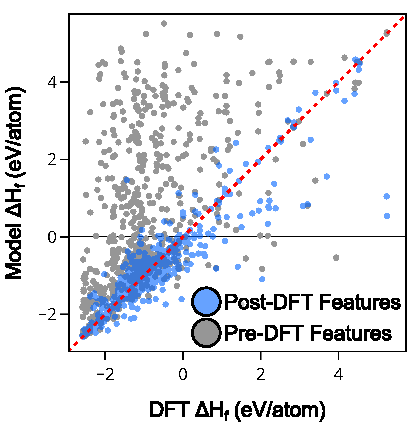
\includegraphics[]
{02_figures/parity_plot/00_al_perf_plot__v1.pdf}}
\caption{\label{fig:parity}
%
Parity plot of the final ML models for \IrOtwo and \IrOthree predicting on either the pre-optimized (grey) or the post-optimized structures of \IrOtwo and \IrOthree.
}
\end{figure*}
% __|
% =========================================================
